\begin{abcliste}
\abc Auf die Boarderin wirken die Gewichtskraft $\vec F_\mathrm{G}$ (nach unten) und die Normalkraft $\vec F_\mathrm{N}$ des Bodens (nach oben); die Reibung wirkt entlang der Bahn und trägt nichts zur Zentripetalkraft bei. Im tiefsten Punkt liegt der Kreismittelpunkt oben. Die Zentripetalkraft ist die Resultierende aus Normalkraft und Gewichtskraft; sie zeigt nach oben, die Normalkraft ist also grösser als die Gewichtskraft. Die Pfeile sind massstäblich gezeichnet:

\begin{center}
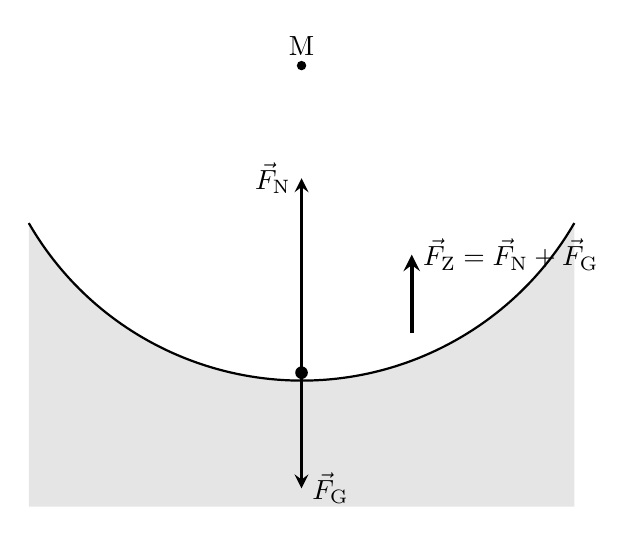
\begin{tikzpicture}[>=stealth]
 \fill[gray!20] (-3.464,2.0) arc (210:330:4) -- (3.464,-1.6) -- (-3.464,-1.6) -- cycle;
 \draw[thick] (-3.464,2.0) arc (210:330:4);
 \fill (0,4) circle (0.06) node[above] {M};
 \fill (0,0.1) circle (0.08);
 \draw[->, very thick] (0,0.1) -- (0,2.57) node[left] {$\vec F_\mathrm{N}$};
 \draw[->, very thick] (0,0.1) -- (0,-1.37) node[right] {$\vec F_\mathrm{G}$};
 \draw[->, ultra thick] (1.4,0.6) -- (1.4,1.6) node[right] {$\vec F_\mathrm{Z} = \vec F_\mathrm{N} + \vec F_\mathrm{G}$};
\end{tikzpicture}
\end{center}

\abc Die Richtung zum Kreismittelpunkt ist positiv. Im tiefsten Punkt der Senke (Mittelpunkt oben) gilt
\begin{align}
 F_\mathrm{N} - m\,g &= \frac{m\,v^2}{r} \\
 F_\mathrm{N} &= \FNsF \\
   &= \mSb\cdot\left(\gE+\frac{\left(\vSb\right)^2}{\rSb}\right) \\
   &= \FNs \approx \result{\FNsP{3}{2}}
\end{align}
Im höchsten Punkt des Buckels liegt der Mittelpunkt unten:
\begin{align}
 m\,g - F_\mathrm{N} &= \frac{m\,v^2}{r} \\
 F_\mathrm{N} &= \FNbF \\
   &= \mSb\cdot\left(\gE-\frac{\left(\vSb\right)^2}{\rSb}\right) \\
   &= \FNb \approx \result{\FNbP{3}{2}}
\end{align}
In der Senke wird sie in den Boden gedrückt, auf dem Buckel ist sie fast schwerelos.

\abc Sie hebt ab, sobald die Normalkraft auf dem Buckel null wird, d.h. wenn die Gewichtskraft allein die Zentripetalkraft liefert: $m\,g = \frac{m\,v^2}{r}$. Die Höchstgeschwindigkeit ist
\begin{align}
 v_\mathrm{max} &= \vSbmF = \sqrt{\gE\cdot\rSb} = \vSbm \approx \result{\vSbmP{0}{2}}
\end{align}
Damit sie auch schneller nicht abhebt, muss sie auf dem Buckel in die Knie gehen (die Beine anziehen): Ihr Körperschwerpunkt bewegt sich dann auf einer flacheren Bahn mit grösserem Krümmungsradius, und wegen $v_\mathrm{max} = \sqrt{g\,r}$ darf sie entsprechend schneller sein.
\end{abcliste}
